\section{Installationsprozess}\label{sec:installationsprozess}

\subsection{Infrastruktur}

Die ViSIT-Applikationen basieren auf der Server-Client-Architektur. Damit diese Applikationen installiert werden können, wird ein hausinternes Netzwerk (Intranet) und ein damit verbundener Server - lokaler Applikations-Server (kurz LAS) - benötigt. Die ViSIT-Applikationen sind in diesem Zusammenhang die Clients, welche über das Netzwerk mit dem lokalen Applikations-Server verbunden sind. Auf dem LAS ist das ViSIT-System installiert, welches über das Internet Zugang zum globalen ViSIT-Netzwerk hat.
Das ViSIT-System ist eine Ansammlung von mehreren kleinen Applikationen, welche parallel auf dem LAS laufen können. Jeder Client, auf welchem eine der ViSIT-Applikationen läuft, hat eigene Server-Software, welche auf dem LAS installiert ist und für die serverseitigen Berechnungen zuständig ist.

Die Applikationen wurden mit der IT-Technologie “Docker” erstellt. Mit Docker hat man die Möglichkeit, Anwendungen in sogenannten Containern auszuführen und diese Container können aufeinander aufbauen und miteinander kommunizieren. Im Gegensatz zu einer virtuellen Maschine, ist eine Docker-basierte Anwendung nur ein Prozess, der auf dem System ausgeführt wird. Es ist somit kein Gastbetriebssystem erforderlich, wie dies bei Virtuellen Maschinen der Falls ist. Container sind einfach konfigurierbare, abgeschlossene Einheiten, in welchen die Anwendung ausgeführt werden. 
Mit Docker können Linux-Container erstellt und verwendet werden können. Die erstellten Container sind eine Virtualisierung auf der Ebene des Betriebssystems. Durch das Erstellen von Containern, werden isolierte Linux-Systeme auf dem gleichen Host erzeugt. Diese Container können flexibel erstellt, bereitgestellt, kopiert und zwischen Umgebungen verschoben werden. Zweck dieser Container ist die Unabhängigkeit und die Fähigkeit, mehrere Prozesse und Applikationen getrennt voneinander betreiben zu können. Die Vorteile von Docker-Containern sind unter anderem Modularität und Versionsverwaltung. Modularität ermöglicht es, bei zum Beispiel einer Reparatur oder Aktualisierung einer Applikation, nur einen Teil dieser Applikation außer Betrieb zu nehmen, ohne die gesamte Applikation außer Betrieb nehmen zu müssen. Docker bietet eine eingebaute Versionsverwaltung, welche es erlaubt, den aktuellen Stand eines Containers in ein sogenanntes Image zu sichern. Somit ist es möglich, die unterschiedlichen Zustände eines Images in einer Historie nachzuverfolgen. Ein Image ist ein Speicherabbild eines Containers und es besteht aus mehreren Layern, welche schreibgeschützt sind und somit nicht verändert werden können. Ein Layer ist wiederum ein Teil eines Images und enthält einen Befehl oder eine Datei, welche dem Image hinzugefügt wurde. Aufgrund dieser Layer kann die ganze Historie eines Images nachvollzogen werden.

\subsection{Projekt auf dem LAS installieren}

Als erster Schritt muss die Datenbank für die Applikation angelegt werden. Wie oben erklärt, wurde für das ViSIT-Projekt Docker verwendet. Damit gespeicherte Daten auch außerhalb eines Containers abgelegt oder in einem anderen Container eingebunden werden können, werden sogenannte Volumes erstellt. Volumes haben viele Vorteile, vor allem aber sind sie einfacher zu sichern oder zu migrieren. Volumes funktionieren sowohl auf Linux- als auch auf Windows-Containern.
Im ersten Schritt wird ein Volume mit der Datenbank auf dem lokalen Rechner im Terminal mit dem Kommando
\begin{lstlisting}[style=MyBashStyle]
docker volume create visit-database
\end{lstlisting} erstellt. Einen eigenen Volume benötigt man deshalb, weil die dort abgelegten Daten permanent gespeichert werden müssen - würde z.B.: der Container gelöscht oder beendet werden - dann wären die nur im Docker Container gespeicherten Daten ebenfalls gelöscht werden. Damit dies nicht passieren kann, werden die Daten parallel lokal auf dem Rechner gespeichert.
Damit Dateien zwischen Geräten in einem lokalen Netzwerk oder zwischen entfernten Geräten über das Internet synchronisiert werden können, wird eine Datensynchronisation mit Peer-to-Peer-Übertragung benötigt. Dies wird im ViSIT-Projekt mit Syncthing realisiert und auch dafür muss ein eigener Volume lokal auf dem Rechner erstellt werden. Dies geschieht mit \begin{lstlisting}[style=MyBashStyle]
docker volume create visit-syncthing
\end{lstlisting}-Befehl, welcher ebenfalls im Terminal ausgeführt wird.
Als nächster Schritt wird das gesamte ViSIT-Projekt von GitHub mittels

\begin{lstlisting}[style=MyBashStyle]
docker run -d --name visit -p 80:80 -p 22000:22000 -p 21027:21027
-v visit-syncthing:/var/syncthing
-v s:/p2p/visit:/var/p2p
-v visit-database:/var/lib/mysql
--restart unless-stopped visitapp/maincontainer \end{lstlisting}

geklont. Beim erstmaligen Starten benötigt der Vorgang länger, da das Projekt aus dem Git Repository sowie das Appbundle (https://github.com/ViSIT-Dev/appbundle) heruntergeladen werden.\\

Erklärung der einzelnen Befehle:\\
\begin{lstlisting}[style=MyBashStyle]
docker run -d --name visit -p 80:80 -p 22000:22000 -p 21027:21027 
\end{lstlisting}

\begin{lstlisting}[style=MyBashStyle]
docker run 
\end{lstlisting}
 startet den Container und mit den mit den Parametern \begin{lstlisting}[style=MyBashStyle]
-d 
\end{lstlisting} gibt man an, dass der Container im Hintergrund dauerhaft laufen soll (Daemonmode). Weiters wird mit \begin{lstlisting}[style=MyBashStyle]
--name visit
\end{lstlisting} der Name des Containers festgelegt, in diesem Fall heißt der Container visit. Der Container kann im weiteren Verlauf auch über diesen Namen angesprochen werden.
Mit dem Parameter
\begin{lstlisting}[style=MyBashStyle]
-p 80:80
\end{lstlisting} werden die Ports vom Host an den Container gebunden. Hier wird der lokale Hostport 80 auf den Containerport 80 gemappt. Die weiteren Ports 
\begin{lstlisting}[style=MyBashStyle]
-p 22000:22000 -p 21027:21027 
\end{lstlisting} werden für das Syncthing und für das Peer to Peer-Netzwerk benötigt.
Als nächstes folgt der Befehl 
\begin{lstlisting}[style=MyBashStyle]
-v visit-syncthing:/var/syncthing
\end{lstlisting}
Mit dem Parameter \begin{lstlisting}[style=MyBashStyle]
-v
\end{lstlisting}
 wird ein Verzeichnis (Volume) auf dem Hostrechner zu einem Verzeichnis innerhalb des Containers verbunden, auf diese Weise werden die Daten persistent gespeichert, das heißt, dass ein Ordner auf dem Hostsystem auf einen Ordner im Container gemappt wird. Das bedeutet, dass die Daten in beiden Ordnern immer inhaltsgleich sind. Ohne dem Mapping zu einen Ordner auf dem Hostsystem, wären alle Daten aus dem Docker Container, wenn dieser Container gelöscht wird, ebenfalls gelöscht. Um die Daten persistent, also dauerhaft zu speichern, wird immer ein Ordner im Hostsystem mit dem entsprechenden Ordner im Docker Container gemappt.
Zuerst wird das Verzeichnis auf dem Hostrechner angegeben, hier \begin{lstlisting}[style=MyBashStyle]
visit-syncthing
\end{lstlisting}
und nach dem Doppelpunkt steht das Verzeichnis innerhalb des Containers, hier \begin{lstlisting}[style=MyBashStyle]
/var/syncthing
\end{lstlisting}

Im nächsten Teil des Befehls \begin{lstlisting}[style=MyBashStyle]
-v s:/p2p/visit:/var/p2p
\end{lstlisting}
 wird ebenfalls zuerst das Verzeichnis auf dem Hostrechner angegeben, \begin{lstlisting}[style=MyBashStyle]
s:/p2p/visit
\end{lstlisting} und dann das Verzeichnis innerhalb des Containers \begin{lstlisting}[style=MyBashStyle]
/var/p2p
\end{lstlisting}
Im nächsten Befehl \begin{lstlisting}[style=MyBashStyle]
-v visit-database:/var/lib/mysql
\end{lstlisting} geht es um die Verbindung zur Datenbank. Hier wird ebenfalls zuerst das Verzeichnis auf dem Hostrechner angegeben \begin{lstlisting}[style=MyBashStyle]
visit-database
\end{lstlisting} und nach dem Doppelpunkt steht das Verzeichnis innerhalb des Containers \begin{lstlisting}[style=MyBashStyle]
/var/lib/mysql
\end{lstlisting}
Zuletzt wird mittels \begin{lstlisting}[style=MyBashStyle]
--restart unless-stopped visitapp/maincontainer
\end{lstlisting} dem System mitgeteilt, dass der Docker Container \begin{lstlisting}[style=MyBashStyle]
visitapp/maincontainer
\end{lstlisting} automatisch gestartet werden soll außer, wenn er manuell oder anderweitig gestoppt wird.

Wenn der Vorgang abgeschlossen ist, kann über Lokalhost im Browser unter \textbf{localhost:80/typo3/} das Backend aufgegerufen werden (siehe Abbildung \ref{img:typo_3_login}). Das erstmalige einloggen in das Backend (TYPO3) erfolgt mit dem \textbf{Benutzername: admin} und \textbf{Passwort: visit-admin}.

\begin{figure}[ht!]
\centering
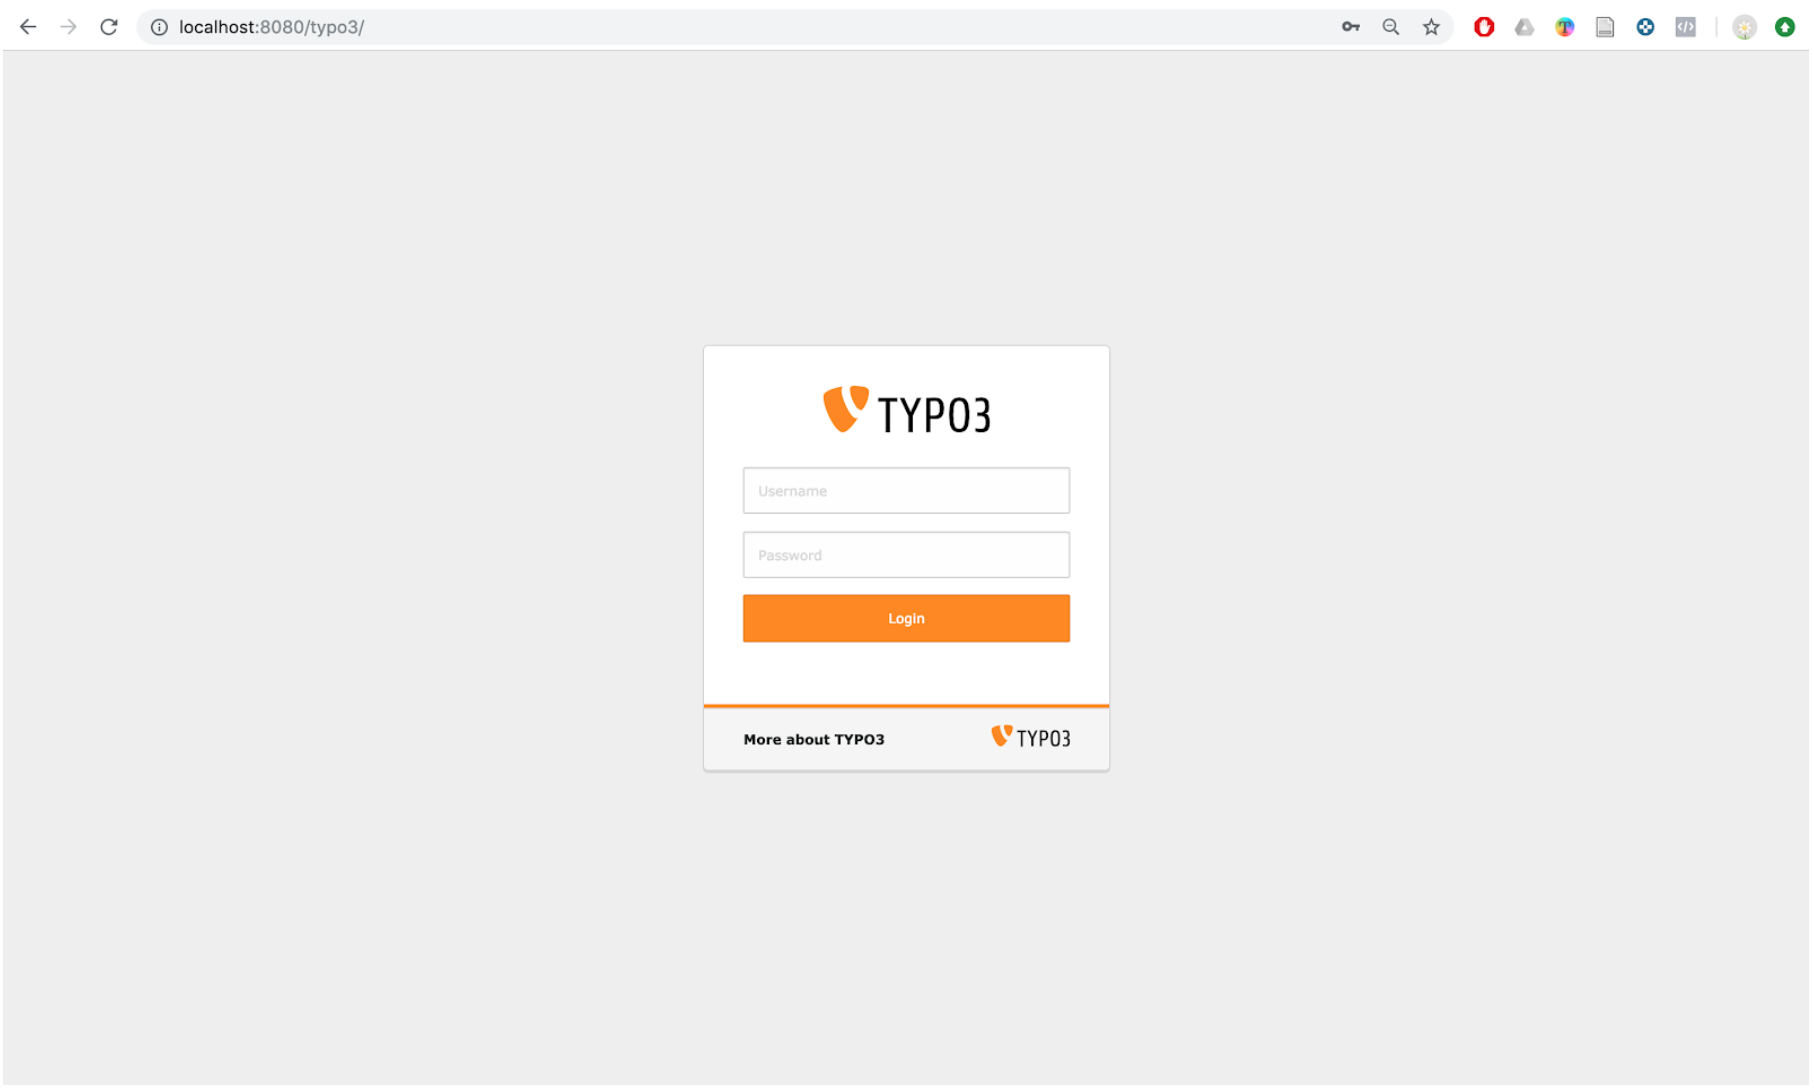
\includegraphics[width=12cm]{Figures/paula/typo_3_login.png}
\caption{Das Login-Fenster für TYPO3 im Browser}
\label{img:typo_3_login}
\end{figure}



\section{TYPO3}
\subsection{Allgemein}

TYPO3 ist ein freies Content-Management-System für Webseiten, es wird in Frontend und Backend getrennt. Als Frontend wird die Präsentationsebene bezeichnet, das ist der Teil einer Applikation, den der Betrachter sehen kann. Als Backend hingegen, bezeichnet man die Datenzugriffsebene, das ist der Teil einer Applikation, welcher nicht für den Besucher sichtbar ist. Das Backend ist der Verwaltungsbereich einer Webseite. TYPO3 wird auf einem Webserver installiert und über den Webbrowser benutzt.

Das Backend ist die Datenzugriffsebene, dieser Teil ist für den Endbenutzer nicht sichtbar. Es beinhaltet die Programmierung einer Applikation und den Administrationsbereich. Im Gegensatz dazu das Frontend, das ist die tatsächliche Webseite, die der Endbenutzer im Browser sieht, also die Benutzeroberfläche.

\subsection{Login}

Damit niemand unbefugter im Frontend sowie Backend etwas verändern kann, muss man sich zuerst ins Backend einloggen. Dies geschieht über den Aufruf der Domain \textbf{localhost:80/typo3/} im Webbrowser (siehe Abbildung \ref{img:typo_3_login}).

\begin{figure}[ht!]
\centering
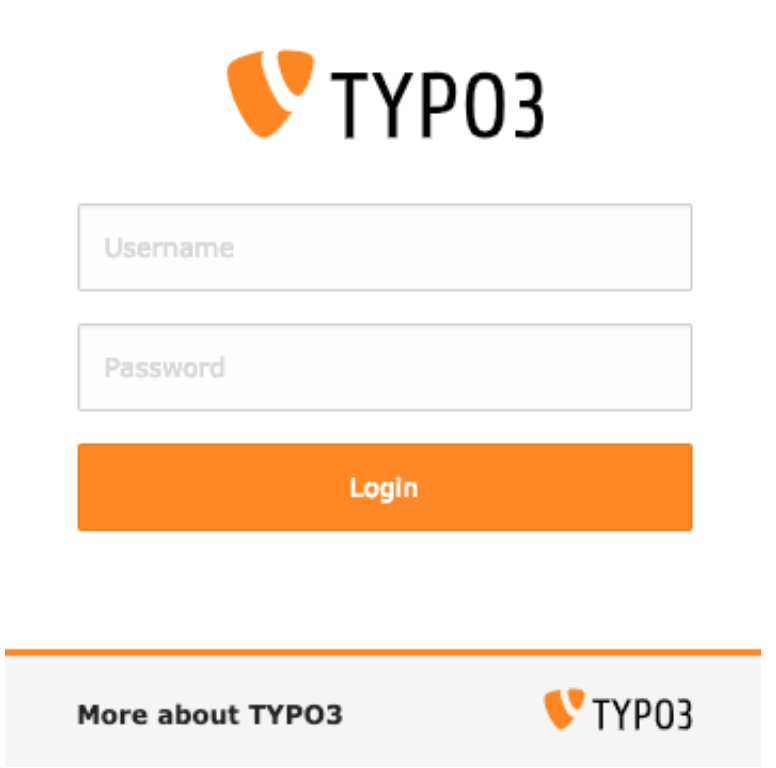
\includegraphics[width=8cm]{Figures/paula/login_TYPO3.png}
\caption{Das Login-Fenster für TYPO3}
\label{img:typo_3_logIn}
\end{figure}

Im Login-Fenster kann der Benutzername sowie das Passwort eingetragen werden (siehe Abbildung \ref{img:typo_3_logIn}). Beim ersten Login ist der \textbf{Benutzername: admin} und das \textbf{Passwort: visit-admin}, dieser muss in weiterer Folge verändert werden. Mehr dazu siehe Anpassung.
Nach einem erfolgreichen Login wird das Backend mit den dazugehörigen Modulen im Browser geladen.

\begin{figure}[ht!]
\centering
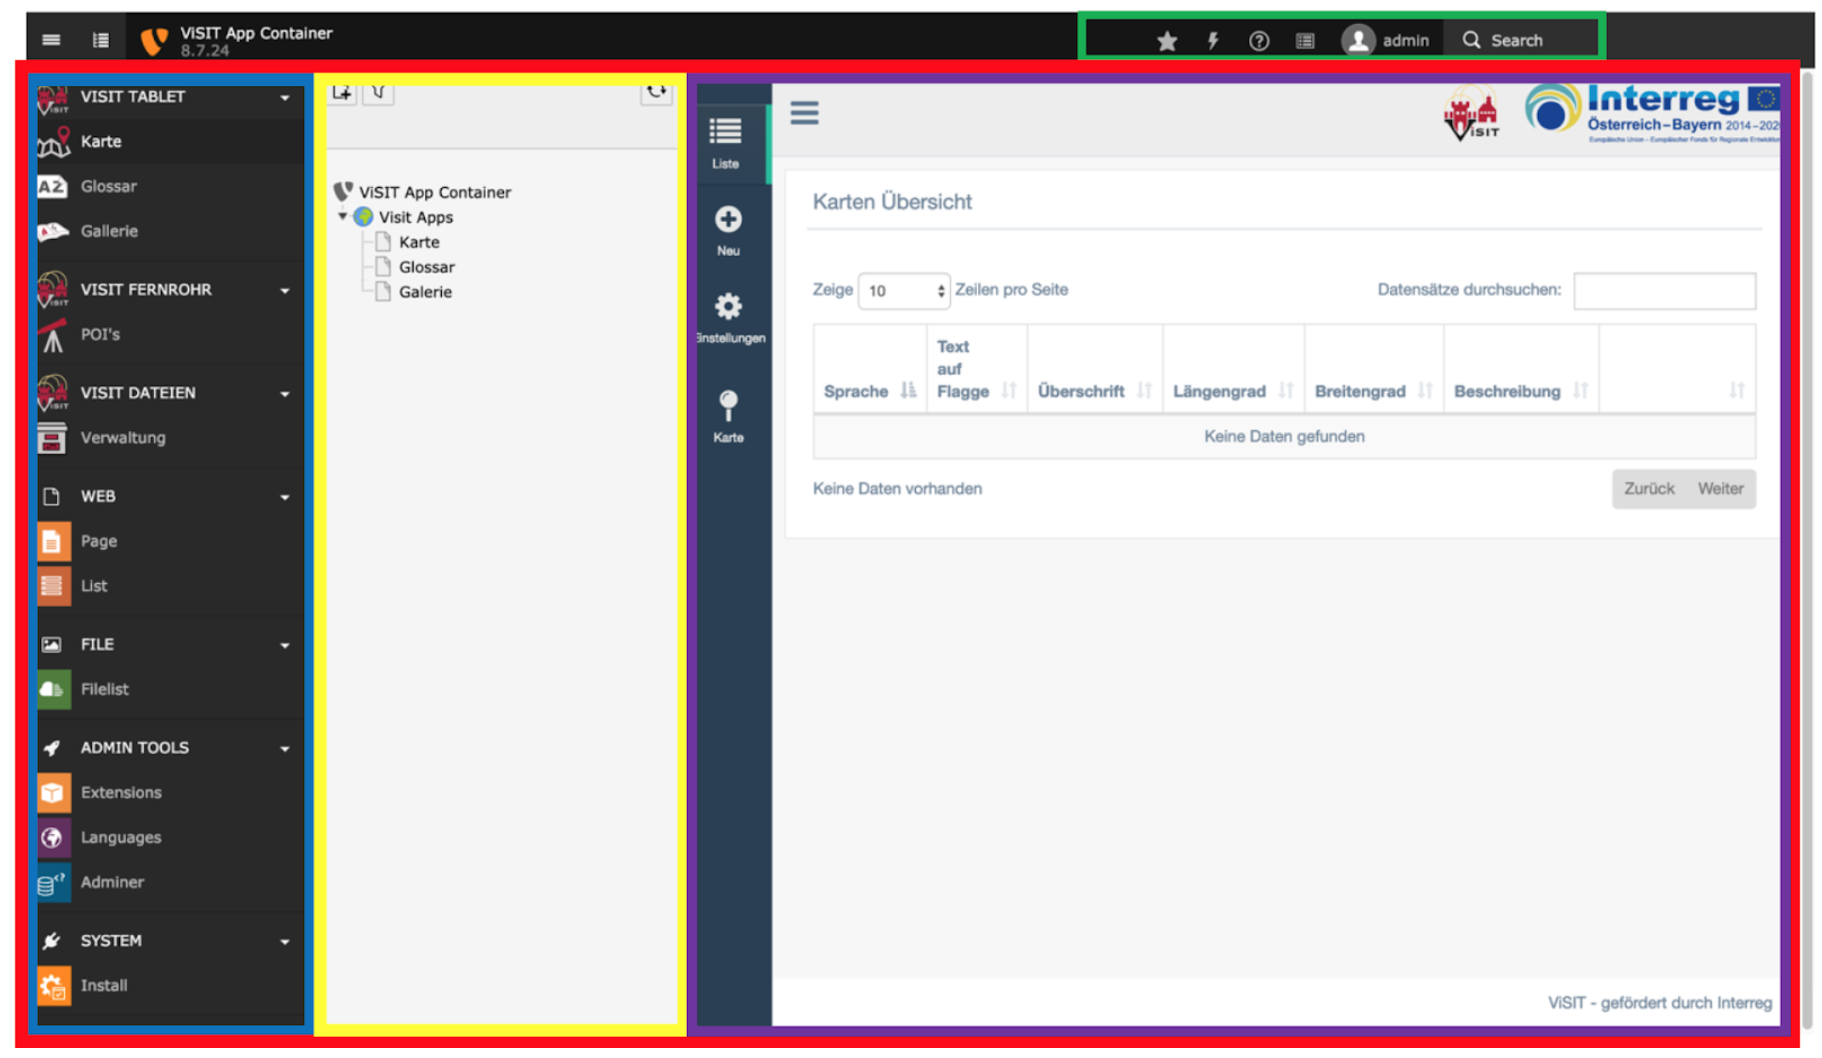
\includegraphics[width=12cm]{Figures/paula/aufbau_TYPO3.png}
\caption{Aufbau des TYPO3-Backends}
\label{img:typo_3_backend}
\end{figure}

\subsection{Aufbau von TYPO3}

Das TYPO3-Backend besteht aus einem Kopfbereich (grün eingerahmt) und einem Hauptbereich (rot eingerahmt), welcher aus drei Spalten besteht (siehe Abbildung \ref{img:typo_3_backend}). Im Kopfbereich kann der Administrator seine TYPO3-Benutzerenstellungen konfigurieren. Im Hauptbereich werden Webdokumente bearbeitet. Das TYPO3-Backend wird von links nach rechts abgearbeitet.

\subsubsection{Kopfleiste}

Die Kopfleiste bietet die Möglichkeit, die im TYPO3 Backend gespeicherten Lesezeichen aufzurufen (Stern-Symbol), den TYPO3 Cache der gesamten Webseite zu leeren (Blitz-Symbol) sowie Hilfe und Dokumentationen (Fragezeichen) zu TYPO3 aufzurufen. Das vierte Symbol zeigt die wichtigsten Systeminformationen. Mit einem Klick auf den Benutzernamen, in der Grafik “admin”, öffnet sich ein Kontext-Menü mit der Möglichkeit Einstellungen an seinem Benutzer vorzunehmen oder sich aus dem TYPO3 Backend auszuloggen. Rechts neben dem Benutzer befindet sich das Suchfeld, mit dem sich das gesamte TYPO3 Backend durchsuchen lässt.

\subsubsection{Die Spalten des Hauptbereichs}

\textbf{Linke Spalte:} \textit{Modulleiste} (blau eingerahmt), hier kann das Modul ausgewählt werden, welches bearbeitet werden soll (siehe Abbildung \ref{img:typo_3_backend}).\\

\textbf{Mittlere Spalte:} \textit{Seitenbaum} (gelb eingerahmt), hier wird die zu bearbeitende TYPO3-Seite ausgewählt. Der Seitenbaum ist das zentrale Element, wenn es darum geht sich durch die Webseite zu navigieren. Hier wird der Aufbau und die Seitenhierarchie der Webseite in einer Struktur abgebildet, die der Ordnerstruktur ähnlich ist. Einzelne Seiten können Unterseiten enthalten, die im Seitenbaum eingerückt dargestellt werden (siehe Abbildung \ref{img:typo_3_backend}).\\

\textbf{Rechte Spalte:} \textit{Arbeitsbereich} (violett eingerahmt), hier wird am ausgewählten TYPO3-Objekt gearbeitet (siehe Abbildung \ref{img:typo_3_backend}).

\subsection{Konfiguration des Backends mit TYPO3}

Die für die Applikationen benötigten TYPO3 Extensions werden automatisch installiert, sollte eine weitere Extension benötigt werden, befindet sich eine Anleitung für die Installation in diesem Abschnitt. Extensions sind optionale Software-Komponenten, also Zusatzmodule, die eine bestehende Software erweitern.\\
Installation von TYPO3 Extensions: Dazu wird in der linken Spalte zuerst das Modul “Extensions” ausgewählt. Dann erscheinen im Hauptfenster verschiedene Extensions, welche alphabetisch gelistet sind. Bei der Erstinstallation werden folgende Extensions (unten ist der Key angegeben, welcher sich in der mittleren Spalte befindet) automatisch installiert (siehe Abbildung \ref{img:extensions}):

\begin{itemize}
    \item visit\_tablets
    \item scheduler
    \item tstemplate
    \item fluid\_styled\_content
    \item setup
\end{itemize}

\begin{figure}[ht!]
\centering
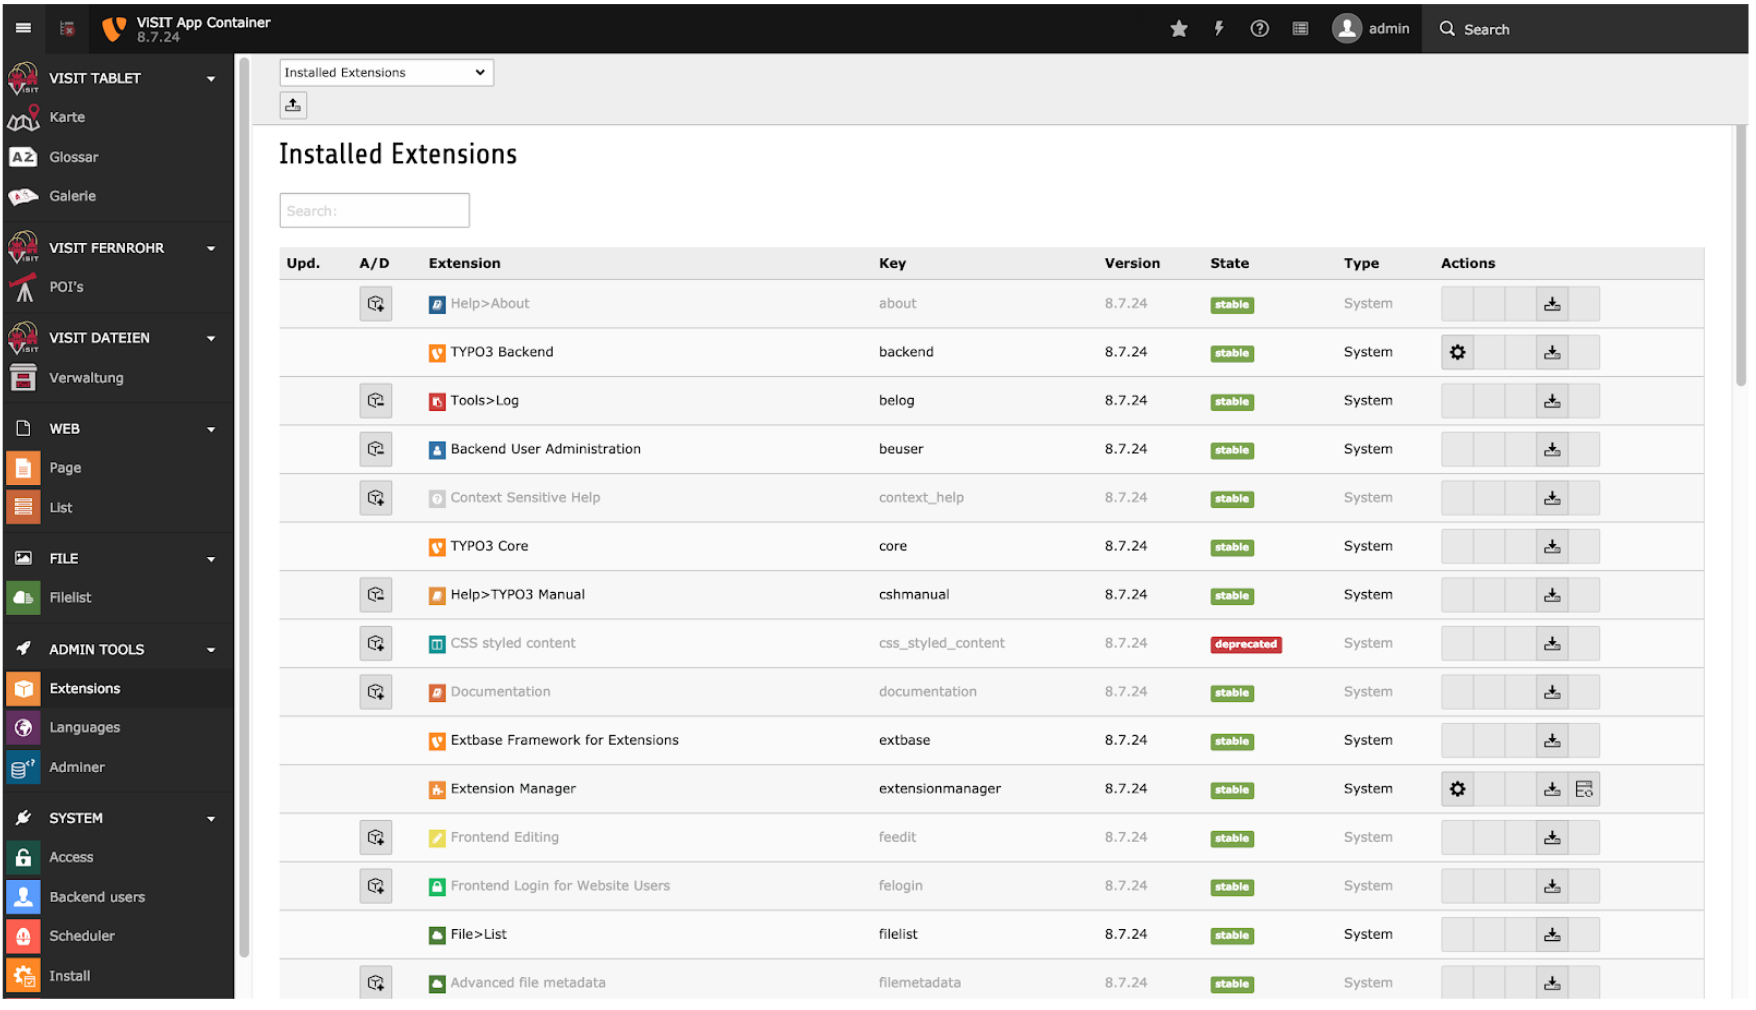
\includegraphics[width=12cm]{Figures/paula/extensions.png}
\caption{Installation der Extensions}
\label{img:extensions}
\end{figure}

Mittels einem Klick auf das Würfelsymbol mit einem Plus werden die oben angegebenen Extensions der Reihe nach aktiviert (siehe Abbildung \ref{img:extensions}). Die aktivierten Extensions erscheinen dann als auswählbare Module in der linken Spalte.
Optional kann im nächsten Schritt die Sprache Deutsch installiert werden, sonst ist die Hauptsprache Englisch. Um die Sprache zu installieren, wird in der linken Spalte unter den ADMIN TOOLS “Languages” ausgewählt (siehe Abbildung \ref{img:sprache_aendern}).

\begin{figure}[ht!]
\centering
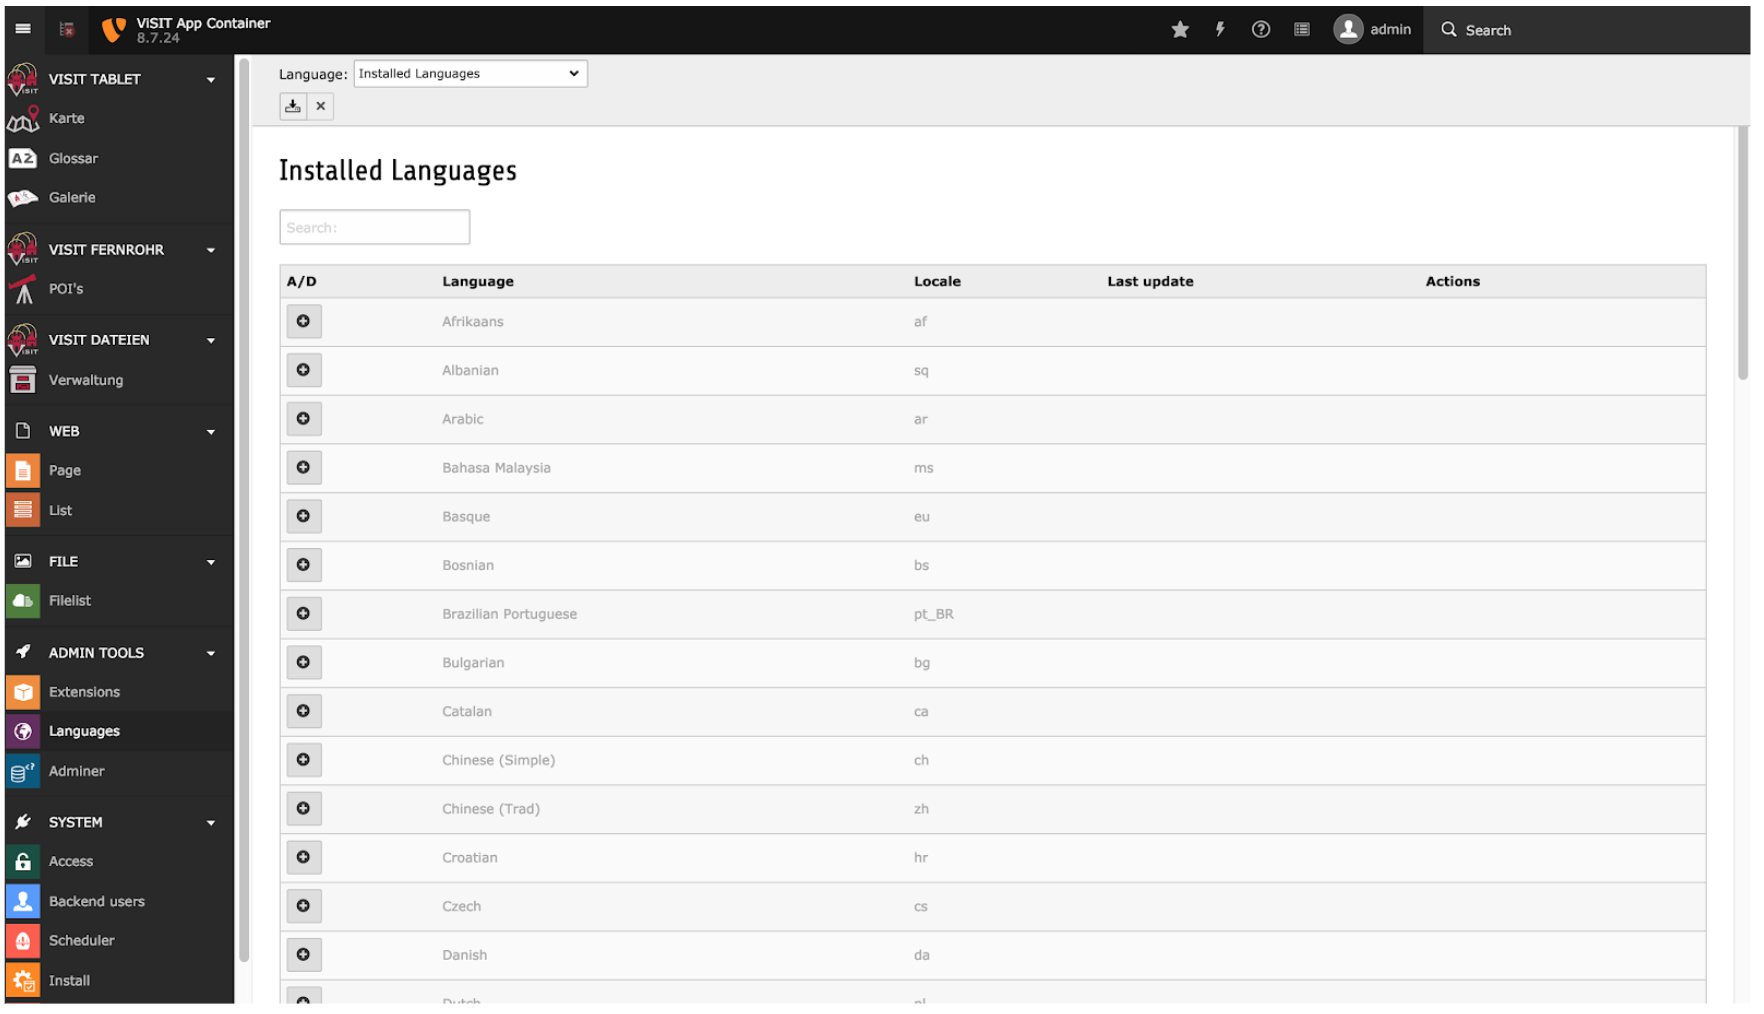
\includegraphics[width=12cm]{Figures/paula/sprache_aendern.png}
\caption{Änderung der Sprache}
\label{img:sprache_aendern}
\end{figure}

Im Hauptfenster erscheinen nach dem Klick die unterstützten Sprachen, hier “German” suchen und zuerst mittels einem Klick auf das Plus-Symbol links von der Sprache die Sprache aktivieren, dabei erscheint oben rechts eine grüne Meldung mit “Success, language was successfully activated.”. Als nächstes muss die aktivierte Sprache mittels Klick auf das Download-Symbol rechts von der Sprache heruntergeladen werden. War der Download erfolgreich, so erscheint oben rechts eine grüne Meldung mit “Success. The translation update has been successfully completed.”.

\subsection{Anpassung}

Im Kopfbereich können die TYPO3-Benutzereinstellungen konfiguriert werden. Dazu wird im Kopfbereich oben rechts zuerst der Benutzer ausgewählt. Bei der Erstinstallation ist es der “admin”, dabei wird ein Menü aufgeklappt, aus welchem die “User settings” ausgewählt werden (siehe Abbildung \ref{img:benutzereinstellungen}).

\begin{figure}[ht!]
\centering
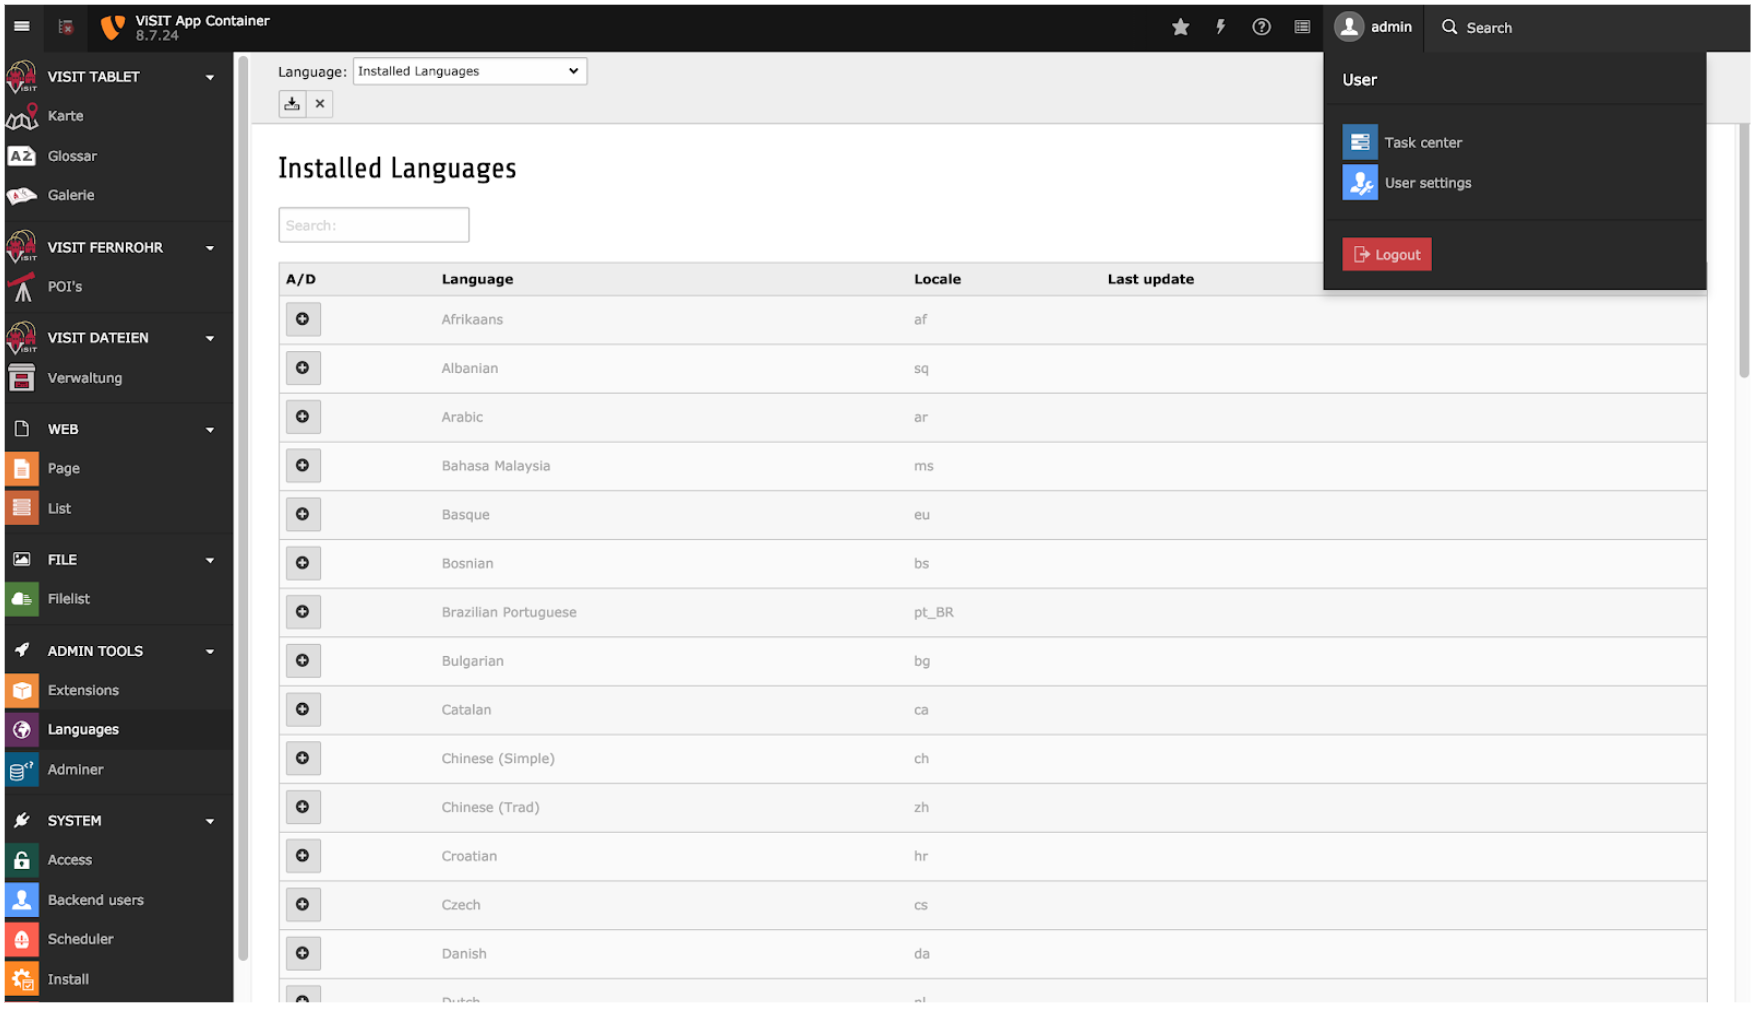
\includegraphics[width=12cm]{Figures/paula/benutzereinstellungen.png}
\caption{Konfiguration der Benutzereinstellungen}
\label{img:benutzereinstellungen}
\end{figure}

Jetzt erscheinen im Hauptbereich die User Settings, welche in dieser Maske konfiguriert werden können. Jetzt kann zuerst die Sprache umgestellt werden. Dies kann gleich im ersten Raster “Personal data”, im unteren Bereich unter Languages geändert werden (siehe Abbildung \ref{img:benutzereinstellungen_sprache}). Hier kann die heruntergeladene Sprache mittels Dropdown ausgewählt werden. Damit die Auswahl auch gespeichert und angewendet wird, muss auf das Speicher-Symbol (Diskette) ganz oben links im Hauptfenster geklickt werden. Nur durch diesen Klick werden die User Settings upgedated und die Sprache auch angewendet. Jetzt erscheinen oben im Hauptfenster drei Meldungen. Die grüne Meldung besagt, dass die Settings upgedated wurden. Die blaue Meldung sagt, dass die Seite (localhost:80/typo3/) neu geladen werden muss, um die Veränderungen zu aktivieren. Die rote Meldung sagt, dass das neue Passwort nicht upgedated wurde, da es nicht zweimal eingegeben wurde.

\begin{figure}[ht!]
\centering
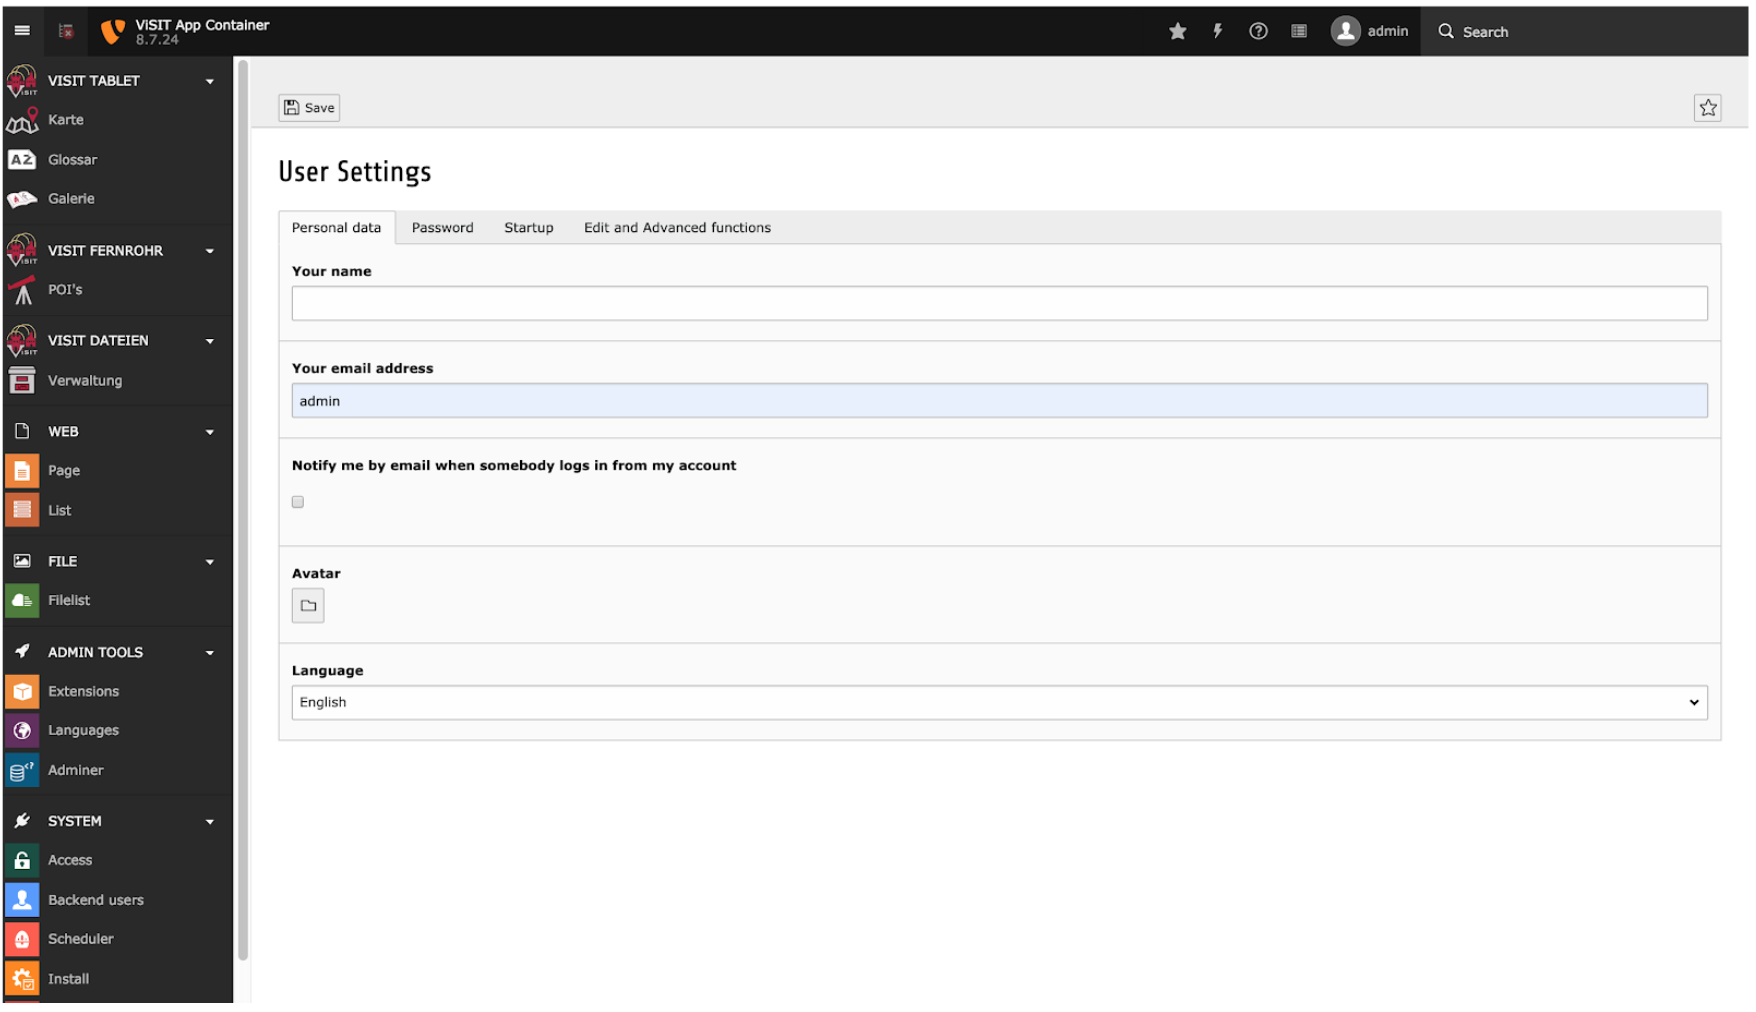
\includegraphics[width=12cm]{Figures/paula/benutzereinstellungen_sprache.png}
\caption{Änderung der Benutzereinstellungen und der Sprache}
\label{img:benutzereinstellungen_sprache}
\end{figure}







\cite{anno4j1}